
\chapter{Graph neural network implementation}

The Graph Neural Network model~\cite{scarselli2009graph} (GNN) is a quite recent (2009) connectionist model, based on recursive neural networks and capable of classifying almost all types of graphs. The main difference between the GNN model and previous connectionist models is the possibility of processing directly nonpositional and cyclic graphs, containing both node labels and edge labels. Although some similar solutions were introduced in an earlier model, the \emph{RNN-LE}~\cite{bianchini2005recursive} in 2005, it was the GNN model that combined several techniques with a novel learning schema to provide a direct and flexible method for graph processing.

\section{Data}
The GNN model is built once for a training set of graphs. In fact, the whole training set can be merged into a large disconnected graph, which can be then fed to the model for learning. For a given dataset each node $n$ is described by a node label $\bm{l}_n$ of fixed size $|\bm{l}_n| \geq 1$. Each directed edge $u \Rightarrow n$ (from node $u$ to node $n$) is described by an edge label $\bm{l}_{(n, u)}$ of fixed size $|\bm{l}_{(n, u)}| \geq 0$. To deal with both directed and undirected edges, the authors propose to include a value $d_l$ in each edge label, denoting the direction of an edge. However, for a maximally general model, in this implementation all the edges were considered as directed. Undirected edges should be thus encoded prior to processing as pairs of directed edges with same labels.

A GNN model can deal with both \emph{graph-focused} and \emph{node-focused} tasks. In graph-focused tasks, for each graph an output $\bm{o}_n$ of fixed size $|\bm{o}_n| \geq 1$ is sought, which can denote e.g. the class of the graph. In the domain of chemistry, where each graph describes a chemical compound, this could describe e.g. the reactivity of a compound. In node-focused tasks, such output $\bm{o}_n$ is sought for every node in every graph. An example of such a task can be the face localisation problem, where for each region of an image the classifier should determine, if it belongs to the face or not. In the rest of this thesis, the \emph{node-focused} task is described, unless stated otherwise.

For this implementation each graph was represented by three .csv files. Each $i$th row of the \emph{nodes file} contained the $i$th node label (comma-separated). Each row of the \emph{edges file} contained information about a directed edge $u \Rightarrow n$: the $u$ node index (row number in nodes file), the $n$ node index and the edge label (comma-separated). Each $i$th row of the \emph{outputs file} contained the $i$th node output (comma-separated). An example is provided in Appendix~\ref{chapter:using}.

\section{Computation units}
The GNN model consists of two computation units, $f_{\bm{w}}$ and $g_{\bm{w}}$, where the $_{\bm{w}}$ subscript denotes the fact that both functions are parametrized by a vector of parameters $\bm{w}$, which is separate for the $f$ and for the $g$ function. The $f_{\bm{w}}$ unit is used for building representation (the \emph{state}) $\bm{x}_n$ of a single node $n$. The $g_{\bm{w}}$ unit is used for generating output $\bm{o}_n$ for a node $n$, basing on its representation $\bm{x}_n$. For a graph-focused task, the representation of the root node is fed to the $g_{\bm{w}}$ function to generate an output for the whole graph. It is important to remind, that for a given classifier there is only one $f_{\bm{w}}$ unit and one $g_{\bm{w}}$ unit (like in the recursive neural network model). All instances of the $f_{\bm{w}}$ unit share their weights and all instances of the $g_{\bm{w}}$ unit share their weights.

Let's denote by $ne[n]$ the neighbors of node $n$, that is such nodes $u$ that are connected to node $n$ by a directed edge $u \Rightarrow n$. Let's further denote by $co[n]$ the set of directed edges pointing from $ne[n]$ towards node $n$ (edges $u \Rightarrow n$). The general forms of $f_{\bm{w}}$ and $g_{\bm{w}}$ functions are defined by equations Eq.~\ref{eq:gnn_f} and Eq.~\ref{eq:gnn_g}, where $\bm{l}_n$ denotes the $n$th node label, $\bm{l}_{co[n]}$ denotes vector of edge labels from $co[n]$ stacked one after another, $\bm{x}_{ne[n]}$ denotes \emph{states} of nodes from $ne[n]$, and $\bm{l}_{ne[n]}$ denotes their labels.

\begin{equation}
\bm{x}_n = f_{\bm{w}}(\bm{l}_n, \; \bm{l}_{co[n]}, \; \bm{x}_{ne[n]}, \; \bm{l}_{ne[n]})
\label{eq:gnn_f}
\end{equation}

\begin{equation}
\bm{o}_n = g_{\bm{w}}(\bm{x}_n, \; \bm{l}_n)
\label{eq:gnn_g}
\end{equation}

\noindent For this implementation, a minimal version of these definitions was chosen, as shown in Eq.~\ref{eq:gnn_fmin} and Eq.~\ref{eq:gnn_gmin}.

\begin{equation}
\bm{x}_n = f_{\bm{w}}(\bm{l}_n, \; \bm{l}_{co[n]}, \; \bm{x}_{ne[n]})
\label{eq:gnn_fmin}
\end{equation}

\begin{equation}
\bm{o}_n = g_{\bm{w}}(\bm{x}_n)
\label{eq:gnn_gmin}
\end{equation}

These forms were chosen to prove that the model is capable of building a sufficient representation of each node. That is, the model should be able to encode the necessary information from a node label $\bm{l}_n$ into the state $\bm{x}_n$. This approach proved to be successful as the first experiment, consisting of a classification task basing on node labels only, yielded perfect results.

From two forms of the $f_{\bm{w}}$ function mentioned in the original article~\cite{scarselli2009graph}, the \emph{nonpositional form} was chosen. The reason was to provide the model with the most general function available, which could deal with both positional and nonpositional graphs. The nonpositional form was also the one yielding better results in the experiments conducted by the authors~\cite{scarselli2009graph}. The equations Eq.~\ref{eq:gnn_ffinal} and Eq.~\ref{eq:gnn_gfinal} show the final equations describing the $f_{\bm{w}}$ and $g_{\bm{w}}$ functions. All instances of the $h_{\bm{w}}$ unit share their weights.

\begin{equation}
\bm{x}_n = \sum_{u \in ne[n]}h_{\bm{w}}(\bm{l}_n, \; \bm{l}_{(n,u)}, \; \bm{x}_{u})
\label{eq:gnn_ffinal}
\end{equation}

\begin{equation}
\bm{o}_n = g_{\bm{w}}(\bm{x}_n)
\label{eq:gnn_gfinal}
\end{equation}

The units $h_{\bm{w}}$ and $g_{\bm{w}}$ were implemented as fully-connected three layer feed-forward neural networks (input lines performing no computation, a single hidden layer and an output layer). For both units the hidden layer consisted of $tanh$ neurons. For the $h_{\bm{w}}$ unit the output layer consisted also of $tanh$ neurons. That's because the output of this unit contributes to the state value and therefore should consist of bounded values only. For the $g_{\bm{w}}$ unit the output layer could consist either of $tanh$ or linear neurons, depending on the values of $\bm{o}_n$ that should be learned.

At this point it's worth noting that the final value of $\bm{x}_n$ is calculated as a simple sum of $h_{\bm{w}}$ outputs. This corresponds to a situation where all the $h_{\bm{w}}$ output values are passed to a neural network in which the set of weights corresponding to a single $h_{\bm{w}}$ input are shared amongst all the $h_{\bm{w}}$ inputs. If we consider that a three layer FNN used as $h_{\bm{w}}$ unit is already an universal approximator, the use of such an additional neural network which just sums all $h_{\bm{w}}$ values using the same shared set of weights is unnecessary. A simple sum should be sufficient and experimental results showed that this assumption stands.

The $f_{\bm{w}}$ and $g_{\bm{w}}$ units are presented in Fig.~\ref{fig:gnn_f} and Fig.~\ref{fig:gnn_g}, where the comma-separated list of inputs stands for a vector obtained by stacking all the listed values one after another.

\begin{figure}[h!]
\begin{center}
	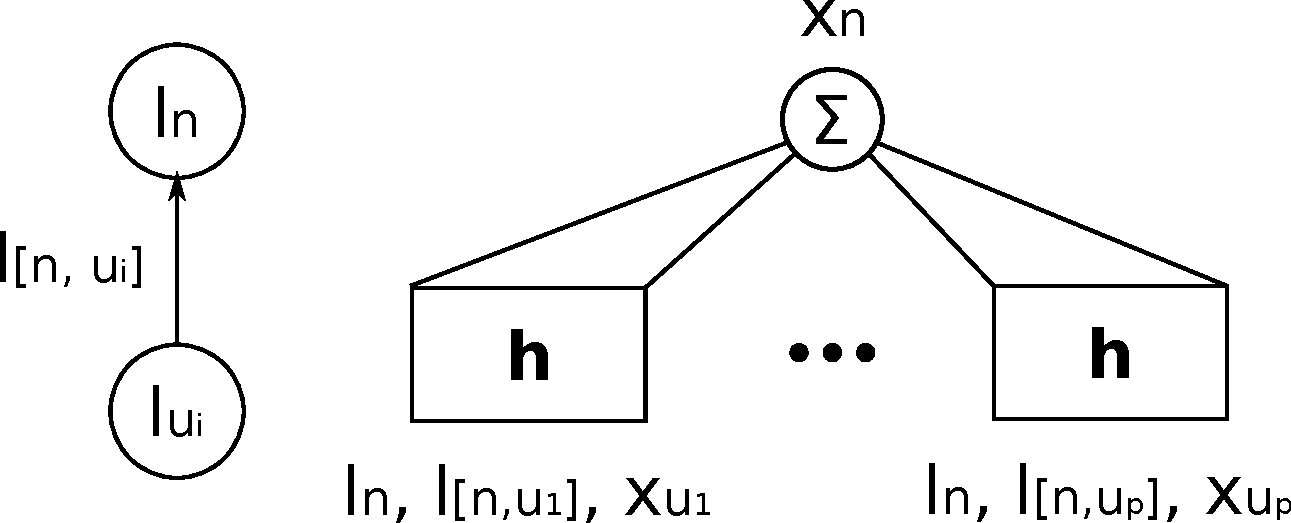
\includegraphics[scale=0.5]{img/f_ext}
	\caption{The $f_{\bm{w}}$ unit for a single node and one of the corresponding edges}
	\label{fig:gnn_f}
\end{center}
\end{figure}

\begin{figure}[h!]
\begin{center}
	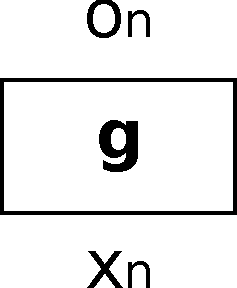
\includegraphics[scale=0.5]{img/g}
	\caption{The $g_{\bm{w}}$ unit for a single node}
	\label{fig:gnn_g}
\end{center}
\end{figure}

The weights of both the $h_{\bm{w}}$ and $g_{\bm{w}}$ units were initialised according to standard neural network practice, to avoid saturation of any $tanh$ activation function: $net_j = \sum_i w_{ij} y_i \in (-1, 1)$, where $net_j$ is the weighted input to $j$th neuron, $y_i$ is the $i$th input value and $w_{ij}$ is the weight corresponding to the $i$th input. The initial input weights of the $g_{\bm{w}}$ unit were divided by an additional factor, i.e. the maximum node indegree of the processed graphs, to take into consideration the fact, that the input of $g_{\bm{w}}$ unit consists of a sum of $h_{\bm{w}}$ outputs. All the input data (node and edge labels) was normalised appropriately before feeding to the model.


\section{Encoding network}
Graph processing by a GNN model consists of two steps: building representation $\bm{x}_n$ for each node and producing an output $\bm{o}_n$. As the representation of a single node depends on other nodes representations, an encoding network for every graph is be built, reflecting the structure of the graph. The encoding network consists of instances of the $f_{\bm{w}}$ unit connected according to the graph connectivity with a $g_{\bm{w}}$ unit attached to every $f_{\bm{w}}$ unit. A sample graph and its encoding network are presented in Fig.~\ref{fig:gnn_encoding}.
It can be seen that, as a cyclic dependence exists in the sample graph, the calculation of the node \emph{states} should be iterative, until at some point convergence is reached.

\begin{figure}[h!]
\begin{center}
	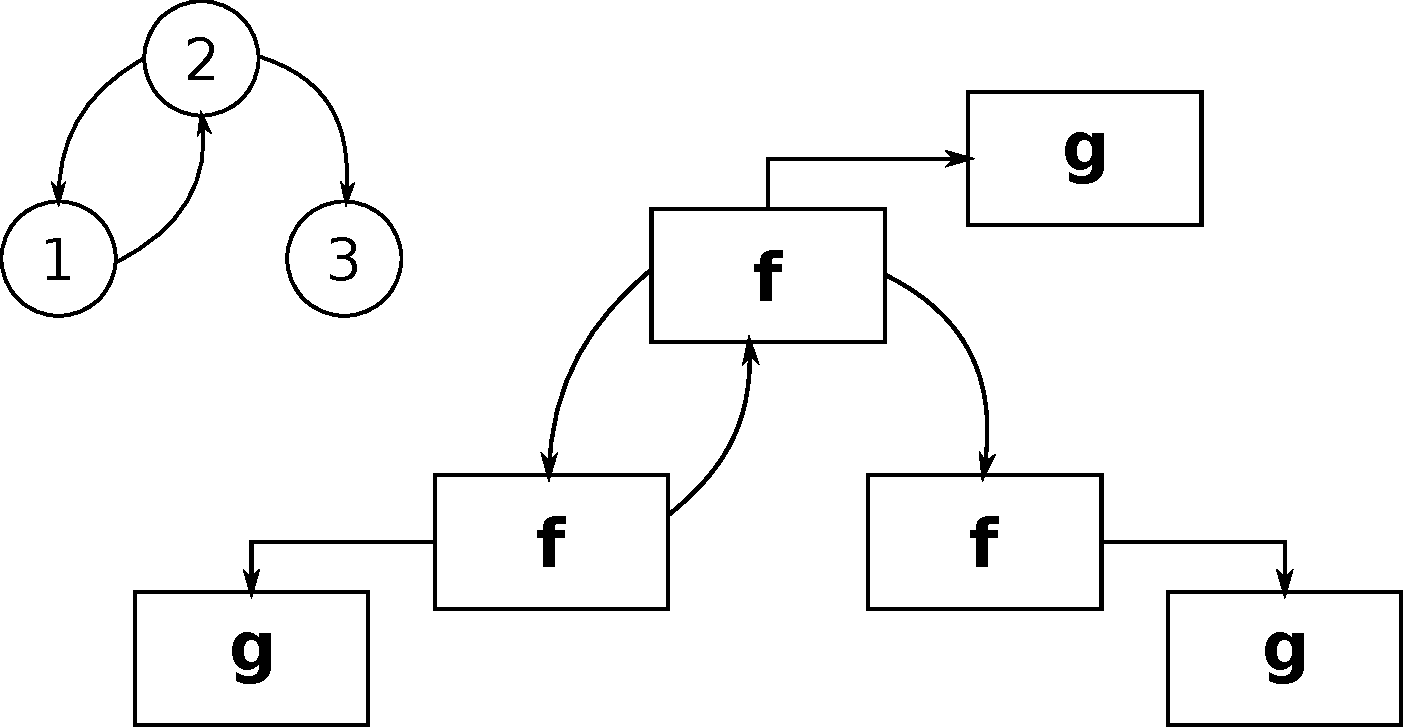
\includegraphics[scale=0.4]{img/encodinginc}
	\caption{A sample graph and the corresponding encoding network}
	\label{fig:gnn_encoding}
\end{center}
\end{figure}


\section{General training algorithm}
Let's denote by $x$ the \emph{global state} of the graph, that is the set of $\bm{x}_n$ for every node $n$ in the graph. Let's denote by $\bm{l}$ and $\bm{o}$ the sets of all labels and all outputs, respectively. Let's further denote by $F_{\bm{w}}$ and $G_{\bm{w}}$ (\emph{global transition function} and \emph{global output function}) the stacked versions of $f_{\bm{w}}$ and $g_{\bm{w}}$ functions, respectively. Now, equations~\ref{eq:gnn_fmin} and~\ref{eq:gnn_gmin} can be rewritten as Eq.~\ref{eq:gnn_fglobal} and Eq.~\ref{eq:gnn_gglobal}.

\begin{equation}
\bm{x} = F_{\bm{w}}(\bm{l}, \; \bm{x})
\label{eq:gnn_fglobal}
\end{equation}

\begin{equation}
\bm{o} = G_{\bm{w}}(\bm{x})
\label{eq:gnn_gglobal}
\end{equation}

\noindent The GNN training algorithm can be described as follows:
\begin{enumerate}
	\item initialize $h_{\bm{w}}$ and $g_{\bm{w}}$ weights
	\item until stop criterion is satisfied:
	\begin{enumerate}
		\item initialize $\bm{x}$ randomly
		\item FORWARD: calculate $\bm{x} = F_{\bm{w}}(\bm{l}, \; \bm{x})$ until convergence
		\item BACKWARD: calculate $\bm{o} = G_{\bm{w}}(\bm{x})$ and backpropagate the error
		\item update $h_{\bm{w}}$ and $g_{\bm{w}}$ weights
	\end{enumerate}
\end{enumerate}


\section{Unfolded network and backpropagation}
To solve the problem of cyclic dependencies, the GNN models adapts a novel learning algorithm for the encoding network. The encoding network is virtually \emph{unfolded} through time until the state $\bm{x}$ converges to a \emph{fixed point} $\hat{\bm{x}} = \bm{x}(t_n)$ of the function  $F_{\bm{w}}$. Then the output $\bm{o}$ is calculated. Such unfolded network for the sample graph is presented in Fig.~\ref{fig:gnn_forward}. Each time step consists of evaluating the $f_{\bm{w}}$ function at every node. What is important, the connections between nodes are taken into consideration only between time steps. In such a way, the problem of cycles ceases to exist and the processed graph can be even fully connected.

\begin{figure}[h!]
\begin{center}
	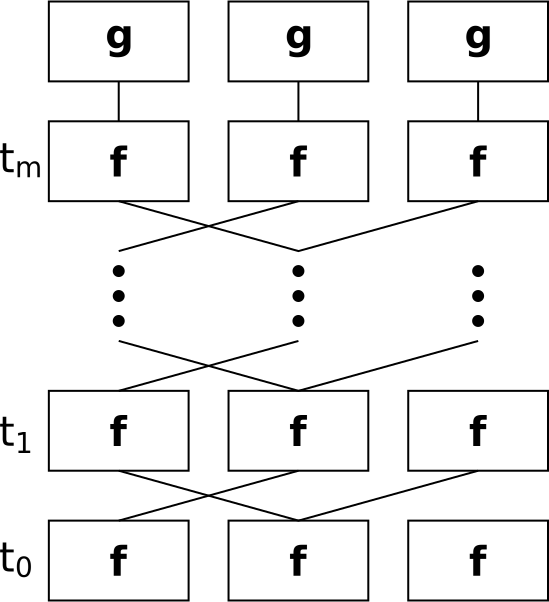
\includegraphics[scale=0.4]{img/forward}
	\caption{Unfolded encoding network for the sample graph}
	\label{fig:gnn_forward}
\end{center}
\end{figure}

After the output $\bm{o}$ is calculated, the error $e_n = (d_n - o_n)^2$ is injected to the corresponding $g_{\bm{w}}$ unit for every node $n$, where $d_n$ denotes the expected node output. The error is backpropagated through the $g_{\bm{w}}$ layer, yielding the value $\frac{\partial e_{\bm{w}}}{\partial \bm{o}}\cdot \frac{\partial G_{\bm{w}}}{\partial x}(\hat{\bm{x}})$. That value is backpropagated through the unfolded network using the BPTT/BPTS algorithm. Additionally, at each time step the $\frac{\partial e_{\bm{w}}}{\partial \bm{o}}\cdot \frac{\partial G_{\bm{w}}}{\partial x}(\hat{\bm{x}})$ error is injected to the $f_{\bm{w}}$ layer, as presented in Fig.~\ref{fig:gnn_backward}. In such a way the error backpropagated through the $f_{\bm{w}}$ layer at time $t_i$ comes from two sources. First, it is the output error of the network $\frac{\partial e_{\bm{w}}}{\partial \bm{o}}\cdot \frac{\partial G_{\bm{w}}}{\partial x}(\hat{\bm{x}})$. Second, it is the error backpropagated through the subsequent time layers of the $f_{\bm{w}}$ unit; in other words, the error backpropagated to node $u$ from all nodes connected with the given node $u$ by an edge $u \Rightarrow n$.

\begin{figure}[h!]
\begin{center}
	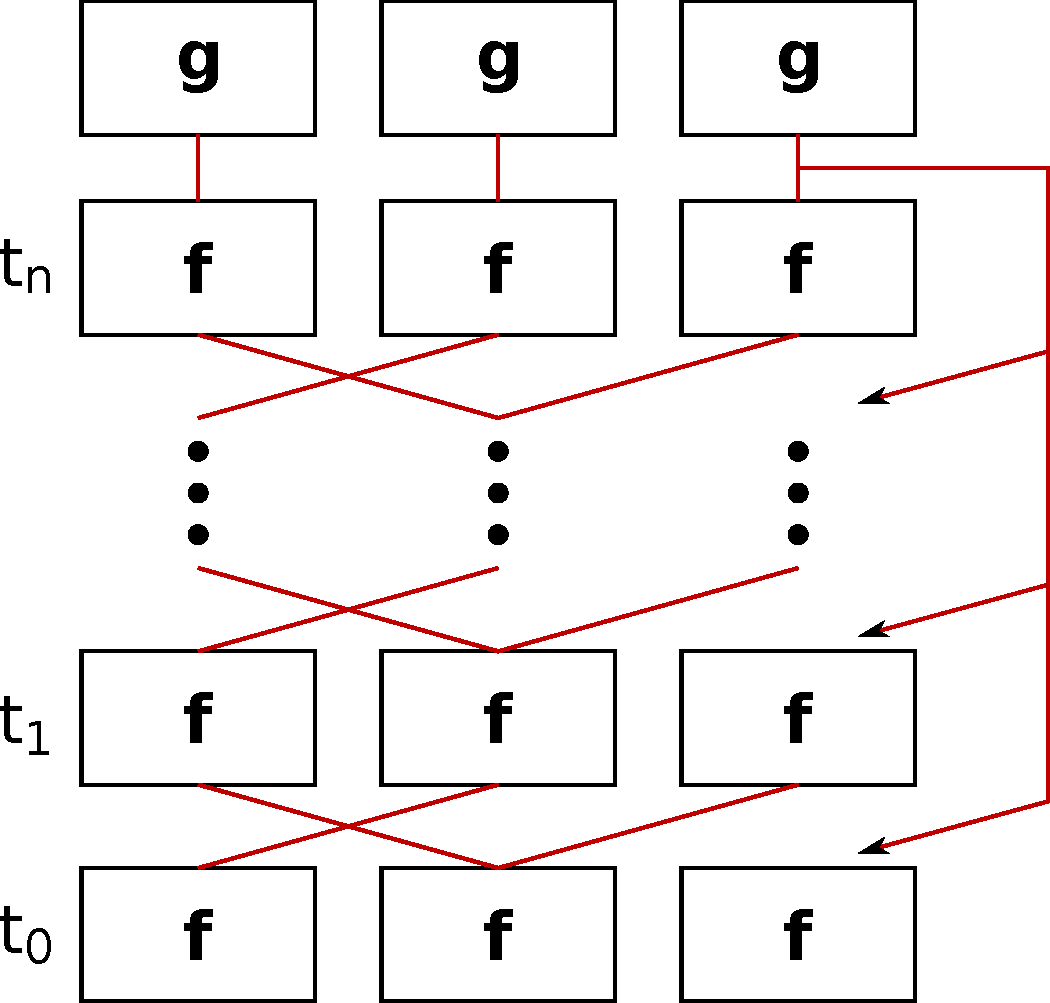
\includegraphics[scale=0.4]{img/backward}
	\caption{Error backpropagation through the unfolded network}
	\label{fig:gnn_backward}
\end{center}
\end{figure}

By injecting the same error $\frac{\partial e_{\bm{w}}}{\partial \bm{o}}\cdot \frac{\partial G_{\bm{w}}}{\partial x}(\hat{\bm{x}})$ at each time step an important assumption is made, which leads to a simplification of the whole backpropagation process. If the state $\bm{x}$ converged to a \emph{fixed point} $\hat{\bm{x}}$ of function $F_{\bm{w}}$ at time $t_n$, then it can be safely assumed that using the value $\hat{\bm{x}}$ at every previous time step $t_i$ instead of the actually used $\bm{x}(t_i)$ would yield the same result at time $t_n$.

Storing the intermediate values of $\bm{x}(t_i)$ and then backpropagating the error using the BPTT/BPTS algorithm would be memory consuming and complicated. However, due to the assumption that $\bm{x}(t_i) = \hat{\bm{x}}$, a different backpropagation algorithm can be used~\cite{scarselli2009graph}, originating from the domain of recurrent neural networks: the Almeida-Pineda algorithm~\cite{pineda1987generalization}~\cite{williams1995gradient}.

Basically, the modified Almeida-Pineda algorithm consists of initializing an \emph{error accumulator} $\bm{z}(0) = \frac{\partial e_{\bm{w}}}{\partial \bm{o}}\cdot \frac{\partial G_{\bm{w}}}{\partial x}(\hat{\bm{x}})$ and then accumulating the error by backpropagating $\bm{z}(j)$ through the $f_{\bm{w}}$ layer until its value converges to $\hat{\bm{z}}$. At each step $j$ the additional error $\frac{\partial e_{\bm{w}}}{\partial \bm{o}}\cdot \frac{\partial G_{\bm{w}}}{\partial x}(\hat{\bm{x}})$ is injected as was shown previously. If the state calculation converged, the error calculation is guaranteed to converge too. The number of iterations needed for the \emph{error accumulator} $\bm{z}$ to converge can be different than the number of time steps needed for the state $\bm{x}$ to converge. In the conducted experiments it was usually much smaller.


\section{Contraction map\label{sec:contraction}}
In the previous paragraphs, it was stated that a fixed point $\hat{\bm{x}}$ of function $F_{\bm{w}}$ is sought. However, how can it be assumed that such a fixed point exists for the function $F_{\bm{w}}$? How to assure that it will be reached by iterating $\bm{x} = F_{\bm{w}}(\bm{x})$ using a random initial $\bm{x}$?

Actually all of the above can be assured by making $F_{\bm{w}}$ a \emph{contraction map}. A \emph{contraction map} (a \emph{non-expansive} map) is a function $F_{\bm{w}}$ for which $d(F_{\bm{w}}(\bm{x}_1), \; F_{\bm{w}}(\bm{x}_2)) \leq d(\bm{x}_1, \; \bm{x}_2)$, where $d(\bm{x}, \; \bm{y})$ is a distance function. For this implementation a distance function $d(\bm{x}, \; \bm{y}) = max_i(|x_{i} - y_{i}|)$ was chosen, as it is independent of the \emph{state} size and therefore, of the number of nodes in a given graph. The \emph{Banach Fixed Point Theorem} states that a contraction map $F_{\bm{w}}(\bm{x})$ has the following properties:
\begin{itemize}
	\item it has a single fixed point $\hat{\bm{x}}$
	\item it converges to $\hat{\bm{x}}$ from every starting point $\bm{x}(t_0)$
	\item the convergence to  $\hat{\bm{x}}$ is exponentially fast~\cite{scarselli2009graph}.
\end{itemize}

\noindent How to assure that $F_{\bm{w}}$, a function composed of neural network instances, is actually a contraction map? The authors propose to impose a penalty function whenever the elements of the Jacobian $\frac{\partial F_{\bm{w}}}{\partial \bm{x}}$ suggest that $F_{\bm{w}}$ isn't a contraction map anymore.

Let $\bm{A} = \frac{\partial F_{\bm{w}}}{\partial \bm{x}}(\bm{x}, \; \bm{l})$ be a block matrix of size $N \times N$ with blocks of size $s \times s$, where $N$ is the number of nodes in the processed graph and $|\bm{x}_n| = s$ is the state size for a single node. A single block $\bm{A}_{n,u}$ measures the influence of the node $u$ on node $n$ if there exists an edge from $n$ to $u$ or is zeroed otherwise. Let's denote by $I_u^j$ the influence of node $u$ on the $j$th element of state $\bm{x}_n$ (Eq.~\ref{eq:gnn_pw_L}). Then the penalty $p_{\bm{w}}$ added to the network error $e_{\bm{w}}$ is defined by Eq.~\ref{eq:gnn_pw}.

\begin{equation}
p_{\bm{w}} = \sum_{u \in N} \sum_{j = 1}^{s} L(I_u^j, \; \mu)
\label{eq:gnn_pw}
\end{equation}

\begin{equation}
L(y, \; \mu) = \left\{
\begin{array}{l l}
	y - \mu		& \quad \text{if $y > \mu$} \\
	0			& \quad \text{otherwise}
\end{array} \right.
\label{eq:gnn_pw_L}
\end{equation}

\begin{equation}
I_u^j =  \sum_{(n, u)} \sum_{i = 1}^{s} |\bm{A}_{n, u}^{i, j}|
\label{eq:gnn_pw_inf}
\end{equation}

According to these equations, the value of $\frac{\partial p_{\bm{w}}}{\partial \bm{w}}$ is calculated and the final error derivative for the $h_{\bm{w}}$ network is calculated as $\frac{\partial e_{\bm{w}}}{\partial \bm{w}} + \frac{\partial p_{\bm{w}}}{\partial \bm{w}}$. It can be seen from Eq.~\ref{eq:gnn_pw_L} that the  term $\frac{\partial p_{\bm{w}}}{\partial \bm{w}}$ affects only those weights that cause an excessive impact and the value of such penalty is proportional to the value of $I_u^j$.

\newpage
\section{RPROP algorithm}
The authors of the GNN algorithm suggest the RPROP algorithm~\cite{riedmiller1993direct} as the weights update algorithm, as an efficient gradient descent strategy. The basic idea of the RPROP algorithm is to use the original weight updates $\frac{\partial e_{\bm{w}}}{\partial \bm{w}}$ only to check their sign. The actual weight updates are calculated by the RPROP algorithm according to the past behaviour of $\frac{\partial e_{\bm{w}}}{\partial \bm{w}}$, which includes fast descent of monotonous gradient slopes, small steps in the proximity of a minimum and reverting updates that caused jumping over a local minimum. Actually, in the case of GNN, the RPROP algorithm should be used not only for its efficiency, but also as a way of dealing with the unpredictable behaviour of the $\frac{\partial p_{\bm{w}}}{\partial \bm{w}}$ term. As the subsequent experiments showed, the value of $\frac{\partial p_{\bm{w}}}{\partial \bm{w}}$ can be larger than the original $\frac{\partial e_{\bm{w}}}{\partial \bm{w}}$ by several orders of magnitude, which could disturb severely the learning algorithm if the RPROP algorithm wasn't used. The RPROP algorithm was implemented using standard recommended values~\cite{riedmiller1993direct}, with the exception of $\Delta_{max}$ which was set to $1$ to avoid large weight changes.


\section{Maximum number of iterations}
As was shown in section~\ref{sec:contraction}, the number of \emph{Forward} or \emph{Backward} steps is finite if $F_{\bm{w}}$ is a contraction map. However, it can be seen, that the penalty imposed on the weights is in fact imposed post factum. Only after the norm of the Jacobian $\frac{\partial F_{\bm{w}}}{\partial \bm{x}}$ increases excessively, the penalty is imposed. This means, that:
\begin{enumerate}
	\item it is not guaranteed that the Jacobian norm will be correct after the penalty is imposed
	\item one \emph{Forward} iteration takes place before the penalty is imposed
\end{enumerate}
Even if the penalty is efficient enough (it isn't necessarily so, as shown in the subsequent experiments), the problem of a \emph{Forward} iteration that may not converge still remains. During experiments it was observed that while usually the number of \emph{Forward} iterations was about 5 to 50, depending on the dataset, from time to time it reached about 2000 iterations or even more (the calculations had to be aborted due to excessive time). To make the calculation time predictable it was necessary to introduce a modification to the original GNN algorithm - a maximum number of \emph{Forward} iterations. The value chosen for the subsequent experiments was 200, as it seemed to be a value large enough in comparison to the standard number of steps reached to assure that the state calculation will converge if $F_{\bm{w}}$ is still a contraction map. If the state calculation doesn't converge, it is not guaranteed that the error accumulation calculation will. Therefore, another similar restriction was introduced for the \emph{Backward} procedure and the maximum number of \emph{Backward} iterations was set to 200. 

\newpage
\section{Detailed training algorithm}
\begin{lstlisting}[mathescape, style=outcode, language=pascal, caption=The learning algorithm]
MAIN
	$\bm{w} = \text{initialize}$
	$\bm{x} = FORWARD(\bm{w})$
	repeat
		$[\frac{\partial eh_{\bm{w}}}{\partial \bm{w}}; \; \frac{\partial eg_{\bm{w}}}{\partial \bm{w}}] = BACKWARD(\bm{x}, \; \bm{w})$
		$\bm{w} = \text{rprop-update}(\bm{w}, \; \frac{\partial eh_{\bm{w}}}{\partial \bm{w}}, \; \frac{\partial eg_{\bm{w}}}{\partial \bm{w}})$
		$\bm{x} = FORWARD(\bm{w})$
	until $\text{satisfied(stop-criterion)}$
	return $\bm{w}$
end

FORWARD($\bm{w}$):
	$\bm{x}(0) = \text{random}$
	$t = 0$
	repeat:
		$\bm{x}(t+1) = F_{\bm{w}}(\bm{x}(t), \; \bm{l})$
		$t = t + 1$
	until $(max_i(|x_i(t + 1) - x_i(t)|) \leq minStateDiff)$ or $(t > maxForwardSteps)$
	return $\bm{x}(t)$
end

BACKWARD($\bm{x}$, $\bm{w}$):
	$\bm{o} = G_{\bm{w}}(\bm{x})$
	$\bm{A} = \frac{\partial F_{\bm{w}}}{\partial \bm{x}}(\bm{x}, \; \bm{l})$
	$\bm{b} = \frac{\partial e_{\bm{w}}}{\partial \bm{o}}\cdot \frac{\partial G_{\bm{w}}}{\partial x}(\bm{x})$
	$\bm{z}(0) = \bm{b}$
	$t = 0$
	repeat:
		$\bm{z}(t - 1) = \bm{z}(t) \cdot \bm{A} + \bm{b}$
		$t = t - 1$
	until $(max_i(|z_i(t - 1) - z_i(t)|) \leq minErrorAccDiff)$ or $(|t| > maxBackwardSteps)$
	$\frac{\partial eg_{\bm{w}}}{\partial \bm{w}} = b$
	$\frac{\partial eh_{\bm{w}}}{\partial \bm{w}} = \bm{z}(t) \cdot \frac{\partial F_{\bm{w}}}{\partial \bm{w}}(\bm{x}, \bm{l}) + \frac{\partial p_{\bm{w}}}{\partial \bm{w}}$
	return $[\frac{\partial eh_{\bm{w}}}{\partial \bm{w}}; \; \frac{\partial eg_{\bm{w}}}{\partial \bm{w}}]$
end
\end{lstlisting}

\section{Graph-focused tasks}
The GNN model can be used for graph-focused tasks by adapting the standard processing algorithm. In a graph-focused task for every graph an output $\bm{o}$ is sought, which is the output of a predefined root node. In such task only the root output error can be measured, as for every other node the expected output is not defined. Thus, the only modification necessary to deal with such a task is to set the error of all non-root nodes to zero. Such a modification was implemented and proved to work well for the modified subgraph matching task (see chapter~\ref{ch:experiments}), where the modified task consisted of determining if a given graph contains the expected subgraph $S$ or not instead of selecting nodes belonging to $S$.
